\documentclass[12pt,a4paper,twoside]{book}
\usepackage{graphicx}
\usepackage{setspace}	%double spacing for text, single for captions, footnotes, etc.
%\usepackage{hypernat} 	%substitut de cite que permet fer hyperlinks
\usepackage{natbib}		% substituye a 'hypernat' que funciona en Windows.
\usepackage[spanish]{babel}
\usepackage[utf8]{inputenc}
\usepackage{color}
\usepackage{hhline} 		% extended styles for tables
\usepackage{multirow}
\usepackage{subfigure}
\usepackage{acronym}
\usepackage{hyperref}
\usepackage{amsmath,amsmath,amssymb} 
\usepackage{fancyhdr}
\usepackage{epsfig, amsmath}
\usepackage{algorithm}
\usepackage{algorithmic}
\usepackage{epigraph}
\usepackage{titlesec}

% general settings
\hypersetup{
	linktocpage=true,
	colorlinks=true,
	linkcolor=blue,
	citecolor=blue,
}
\definecolor{Hgray}{gray}{0.6}

\newenvironment{definition}[1][Definition]{\begin{trivlist}
\item[\hskip \labelsep {\bfseries #1}]}{\end{trivlist}}

\setlength{\topmargin}{0cm}
\setlength{\textheight}{23cm}
\setlength{\textwidth}{17cm}
\setlength{\oddsidemargin}{0cm}
\setlength{\evensidemargin}{0cm}
\setlength{\headheight}{1cm}

% indica que las 'sub-sub-sections' sean numeradas y aparezcan en el indice
\setcounter{secnumdepth}{3}
\setcounter{tocdepth}{2}

% settings for code
\renewcommand{\algorithmicrequire}{\textbf{Entrada: }}
\renewcommand{\algorithmicensure}{\textbf{Salida: }}
\newcommand{\sectionbreak}{\clearpage}

%%%%%%%%%%%%
% DOCUMENT %
%%%%%%%%%%%%
\begin{document}

% portada
\newpage
\thispagestyle{empty}

\baselineskip 2em

%\vspace*{1cm}

\centerline{
\includegraphics[width=0.6\textwidth]{images/UOC-logo}}
\begin{center}
\textsc{Universitat Oberta de Catalunya (UOC) \\
 Máster Universitario en Ciencia de Datos (\textit{Data Science})\\}

%\centerline {\pic{UOC}{4cm}}

\vspace*{1.5cm}

\textsc{\Large TRABAJO FINAL DE MÁSTER}

\vspace*{0.5cm}

\textsc{\large Área: Minería de datos y Machine Learning}


%\textbf{\Huge VirtualTechLab Model: }

\vspace*{2.0cm}

\textbf{\Large Detección de anomalías en entorno del Internet de las cosas}


\vspace{2.5cm}
\baselineskip 1em

\baselineskip 2em
-----------------------------------------------------------------------------\\
Autor:      Gonzalo Pedro Mellizo-Soto Díaz\\
Tutor:      Carlos Hernández Gañán \\
Profesor:   Jordi Casas Roma \\
-----------------------------------------------------------------------------\\
\vspace*{1.5cm}
Madrid, \today

\end{center}

\newpage
\pagestyle{empty}
\hfill

\newpage
% abstract
\pagenumbering{roman} 
\setcounter{page}{1} 
\pagestyle{plain}

%%%%%%%%%%%%%%%%
%%% CREDITOS %%%
%%%%%%%%%%%%%%%%
\chapter*{Copyright}

\vspace{1cm}

\begin{figure}[ht]
    \centering
	
\includegraphics[scale=1]{images/license.png}
\end{figure}

Esta obra está sujeta a una licencia de Reconocimiento -  NoComercial - SinObraDerivada

\href{https://creativecommons.org/licenses/by-nc-nd/3.0/es/}{3.0 España de CreativeCommons}.

%%%%%%%%%%%%%
%%% FICHA %%%
%%%%%%%%%%%%%
\chapter*{FICHA DEL TRABAJO FINAL}

\begin{table}[ht]
	\centering{}
	\renewcommand{\arraystretch}{2}
	\begin{tabular}{r | l}
		\hline
		Título del trabajo: & Detección de anomalías en el entorno del Internet de las cosas\\
		\hline
        Nombre del autor: & Gonzalo Pedro Mellizo-Soto Díaz\\
		\hline
        Nombre del colaborador/a docente: & Carlos Hernández Gañán\\
		\hline
        Nombre del PRA: & Jordi Casas Roma\\
		\hline
        Fecha de entrega (mm/aaaa): & 06/2019\\
		\hline
        Titulación o programa: & Máster Universitario en Ciencia de Datos\\
		\hline
        Área del Trabajo Final: & Minería de datos y Machine Learning \\
		\hline
        Idioma del trabajo: & Español\\
		\hline
        Palabras clave & Machine Learning, IOT, Anomaly Detection\\
		\hline
	\end{tabular}
\end{table}

%%%%%%%%%%%%%%%%%%%
%%% DEDICATORIA %%%
%%%%%%%%%%%%%%%%%%%
\chapter*{Cita}

\setlength\epigraphwidth{.8\textwidth}
\setlength\epigraphrule{0pt}

\epigraph{\itshape``Nuestro lema es: más humanos que los humanos"}{Eldon Tyrell, \textit{Blade Runner}}

%%%%%%%%%%%%%%%%%%%
%%% Agradecimientos %%%
%%%%%%%%%%%%%%%%%%%
\chapter*{Agradecimientos}

TO BE DEFINED

Si se considera oportuno, mencionar a las personas, empresas o instituciones que hayan contribuido en la realización de este proyecto.

%%%%%%%%%%%%%%%%
%%% RESUMEN  %%%
%%%%%%%%%%%%%%%%
\chapter*{Abstract}
\addcontentsline{toc}{chapter}{Abstract}

\onehalfspacing

In recent years the amount of connected devices has greatly increased, with an increasing number of applications in the industry each day. This devices can be subject of attacks causing instability or data leaks that can be dangerous both for the users and the enterprises, in order to avoid or confront them, security and early detection are becoming a must in a connected world. The focus is the monitoring and detection of the attacks in Internet of Things devices using state of the art Machine Learning techniques. Models such as SVM, DBScan or Isolation Forests have been used and assembled in order to identify with a better accuracy when an attack is happening. With this assembly, attack detection has increased up to 15\% comparing to traditional methods and individual model usages and times have been considerably reduced. An active use of Machine Learning models has shown a great improvement at anomaly detection by securing the devices and decreasing the reaction times when facing attacks.

\vspace{0.5cm}

Durante los últimos años se encuentra una creciente cantidad de dispositivos conectados entre sí, cada vez con más aplicaciones en la industria. Estos dispositivos pueden ser atacados y provocar inestabilidad o una fuga de datos, por lo tanto la protección y la pronta detección de ataques y/o anomalías es vital en un mundo cada vez más conectado. El objetivo es la monitorización y detección de estos ataques en dispositivos del \textit{Internet of Things} utilizando técnicas del estado del arte de Machine Learning para su detección y poder así responder con una mayor rapidez a los ataques. Para la detección se han utilizado modelos estadísticos, como SVM, DBScan o Isolation Forests, que en su conjunto permitan identificar con mayor precisión cuando se está produciendo un ataque. El conjunto de la clusterización con la clasificación de puntos anómalos muestra una mayor robustez, frente al uso individual de cada uno de los modelos aumentando la detección en hasta un 15\%. Se demuestra cómo el uso de los modelos permite proteger los dispositivos y mejorar la seguridad al disminuir los tiempos de reacción frente a los ataques.

\vspace{0.5cm}
\textbf{Palabras clave}: Machine Learning, IOT, Anomaly Detection
\newpage

\pagestyle{fancy}
\renewcommand{\chaptermark}[1]{ \markboth{#1}{}}
\renewcommand{\sectionmark}[1]{\markright{ \thesection.\ #1}}
\lhead[\fancyplain{}{\bfseries\thepage}]{\fancyplain{}{\bfseries\rightmark}}
\rhead[\fancyplain{}{\bfseries\leftmark}]{\fancyplain{}{\bfseries\thepage}}
\cfoot{}

% indice
\cleardoublepage
\phantomsection
\addcontentsline{toc}{chapter}{Índice}
\tableofcontents
% listado de figuras
\cleardoublepage
\phantomsection
\addcontentsline{toc}{chapter}{Llistado de Figuras}
\listoffigures
% listado de tablas
\cleardoublepage
\phantomsection
\addcontentsline{toc}{chapter}{Listado de Tablas}
\listoftables

\thispagestyle{empty}

\pagenumbering{arabic}

\pagestyle{fancy}
\renewcommand{\chaptermark}[1]{ \markboth{#1}{}}
\renewcommand{\sectionmark}[1]{\markright{ \thesection.\ #1}}
\lhead[\fancyplain{}{\bfseries\thepage}]{\fancyplain{}{\bfseries\rightmark}}
\rhead[\fancyplain{}{\bfseries\leftmark}]{\fancyplain{}{\bfseries\thepage}}
\cfoot{}

\onehalfspacing

% capitulos del documento
\chapter{Introducción}
\label{chapter:introduccion}


%%% SECTION
\section{Contexto y justificación del Trabajo}
Cada vez se encuentran más dispositivos conectados entre sí no solo en la industria, si no también en los hogares, esta conexión entre dispositivos los hace vulnerables a ataques informáticos que pueden afectar en gran medida a los usuarios, no solo pueden provocar un mal funcionamiento de los mismos, si no que también puede provocar la fuga de datos de distinta sensibilidad. La previsión en los futuros años es de cada vez estar más conectados y una pronta detección de los ataques puedo ayudar a evitar los problemas derivados de los mismos, mediante una pronta reacción o frente a la previsión de un ataque.

\vspace{0.5cm}

Actualmente se utilizan distintas medidas de seguridad como control de acceso físico al dispositivo, encriptación de datos, firewalls, securización de red, etc... Sin embargo, en muchos casos la detección de anomalías aplican un umbral estacionario, provocando que en el caso de un ataque ya sea demasiado tarde para reaccionar o no sean capaz de identificar patrones extraños previos al ataque. Con la aplicación de nuevas técnicas se pretende mejorar los tiempos de reacción e incluso predecir cuándo puede suceder un ataque.

\section{Explicación de la motivación personal}
La razón principal de la selección del proyecto es la posibilidad de aprender y utilizar técnicas de Machine Learning en un sector desconocido que permita diversificar conocimientos. Cada vez más todo se encuentra conectado e investigar cómo clasificar cuando se está produciendo un ataque permite profundizar en conocimientos de seguridad y aplicarlos en un problema real.

\vspace{0.5cm}

La aplicación de técnicas en un problema real ayuda a comprender mejor el uso de las herramientas y el por qué y cuándo se deben de utilizar. De este modo, se añade un nuevo conocimiento que puede aportar en el ámbito profesional y puede utilizarse también en un entorno privado.


\section{Objetivos del Trabajo}
Los objetivos del trabajo son los siguientes:

\begin{itemize}
  \item Adquisición de conocimiento del sector y de los dispositivos IOT
  \item Lectura y comprensión de las técnicas del estado del arte en detección de anomalías en dispositivos conectados.
  \item Obtención de datos reales de conexiones a dispositivos IOT, en caso de no ser posible, generación de datos sintéticos.
  \item Prueba de las técnicas encontradas y evaluación en el problema actual.
  \item Investigación de algoritmos tradicionales de Machine Learning y su utilidad en el problema actual.
  \item Desarrollo de la solución utilizando los algoritmos más aptos.
  \item Evaluación de la detección de patrones y ataques de las técnicas utilizadas.
  \item Comparar los resultados obtenidos con el estado del arte y probar si existen mejoras frente a los métodos actuales.
\end{itemize}

\section{Descripción general del problema}

En la actualidad, la cantidad de dispositivos informáticos existentes que pueden ser víctimas de un ataques es masiva, por lo que securizar bien los dispositivos es fundamental. A pesar de el uso de distintos protocolos de seguridad, se generan nuevos tipos de ataque todos los días, por lo tanto la detección es una necesidad para evitar los problemas derivados.

\vspace{0.5cm}

La pérdida de control de los dispositivos o la fuga de información de los mismos puede provocar pérdidas millonarias a las empresas o provocar una gran inseguridad a los usuarios de productos IOT, así como provocar posibles daño a infraestructuras o personas. Por otro lado, muchos de los dispositivos pueden no tener la capacidad de computación necesaria para incluir una capa de seguridad robusta, que puede compensarse con una detección temprana. 


\section{Enfoque y método seguido}
El enfoque es aplicado al conocer el problema y se intenta dar respuesta a preguntas específicas, mediante la aplicación de los conocimientos obtenidos y la evaluación de la propia aplicación de los mismos.  \par

\vspace{0.5cm}

El método seguido del desarrollo se va a implementar dentro del marco de trabajo \textit{Agile} pensando el desarrollo de la solución como un producto, de este modo se podrá iterar sobre una arquitectura definida y enfocarse en el desarrollo del producto en su total, frente a un modelo tradicional de cascada donde cada fase de desarrollo recae en una sola parte del total.

\vspace{0.5cm}

El formato de entrega será mediante un \textit{minimum viable product} (MVP) en sprints de dos semanas durante el periodo de desarrollo y evaluación de las necesidades según la evolución del producto.

\section{Planificación del Trabajo}

Para la planificación del trabajo se han subdividido las tareas principales y se han mostrado en el siguiente diagrama de Gantt \ref{fig:gantt}.

\begin{itemize}
    \item Pec01 - Definición
    \item Pec01 - Planificación
    \item Pec02 - Búsqueda de fuentes del estado del arte
    \item Pec02 - Lectura de estado del arte
    \item Pec02 - Justificación de estado del arte
    \item Pec02 - Redacción
    \item Pec02 - Refinamiento de objetivos
    \item Pec03 - Planificación de Sprints
    \item Pec03 - Sprint 1
    \item Pec03 - Sprint 2
    \item Pec03 - Sprint 3
    \item Pec03 - Refinamiento/Redacción
    \item Pec04 - Revisión apartados anteriores
    \item Pec04 - Redacción nuevos apartados
    \item Pec05 - Presentación y defensa
\end{itemize}



\begin{figure}[h]
	\centering
	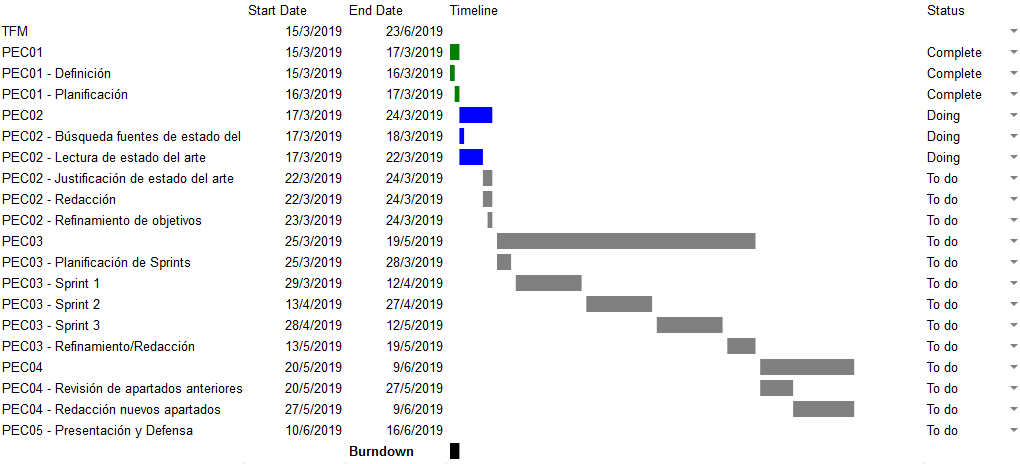
\includegraphics[width=1\textwidth]{figs/gantt_init.PNG}
	\caption{Planificación de tareas}
	\label{fig:gantt}
\end{figure}


% bibliografia
\addcontentsline{toc}{chapter}{Bibliografía}
\bibliographystyle{plain}
\bibliography{referencias}

\end{document}